\section{Technical Information}
\label{sec:Tech}



This section will provide a general idea of the different systems used to create the Web Application. The following items summarize important technical information of the project.

\begin{itemize}

\item What technologies did you use to set up the front-end? Python, Pandas, Dash libraries, GeoJSON files (Colombian map), html,css
\item What types of visualizations do you display and why?
A General Colombian Map with information associated to the risks, number of death,  number of people and houses affected. A Detailed map but with information that correspond to the political division and subdivision.
\item How does the Dashboard pass and receive information for use from the AWS-hosted
components? views and database queries were created. This to create pandas DataFrames that are used to generate the information presented in the front end.

\item What computation tool did you use? an EC2 Linux Ubuntu instance
\item Code / program design paradigms used: Standard Python Dash application with callbacks  with CSS, also to embed the  page on HTML page with an Iframe.


\end{itemize}




\subsection{AWS-hosted database}

Figure \ref{fig:er_model} shows the entity relationship model of the project. The information contained in the model is:

\begin{enumerate}

\item Disasters : information of disasters of Colombia from 1998 to 2017, with the following fields: date,  Colombian political division, number of disasters, death, injuries, missing people, families, houses, public and education services infrastructures and some economical  information. (table disasters)
\item Events: name and category of the event (table eventos)
 
\item Political division of Colombia (divipola): ID of division, subdivision and name of both (divipola table)

\item Population estimates: relates population by period, age groups, political division, id, and gender

\item Weather estimates:  weather information from 1990 to 2018 (minimal temperatures, maximal temperatures, precipitations) (tables: historico\_cond\_metereologicas, load\_mintemp, load\_maxtemp, load\_precipitaciones)	


\item Load tables: temporal tables for loading disasters, political division, population (tables: load\_disasters, load\_divipola, load\_populations)

\item Views: wv\_disasters (summary table for disasters). 

\end{enumerate}

The SQL script for the creation of the database on AWS can be download from this link: \\ \url{https://marioceron-case-51.s3.amazonaws.com/final_project/Script_Desastres_DB.sql}{}

Full backup Database: \\ 
\url{https://marioceron-case-51.s3.amazonaws.com/final_project/Script_Desastres_DB_full.sql}{} \\ \\ 


 
\begin{figure}[!htb]
\center{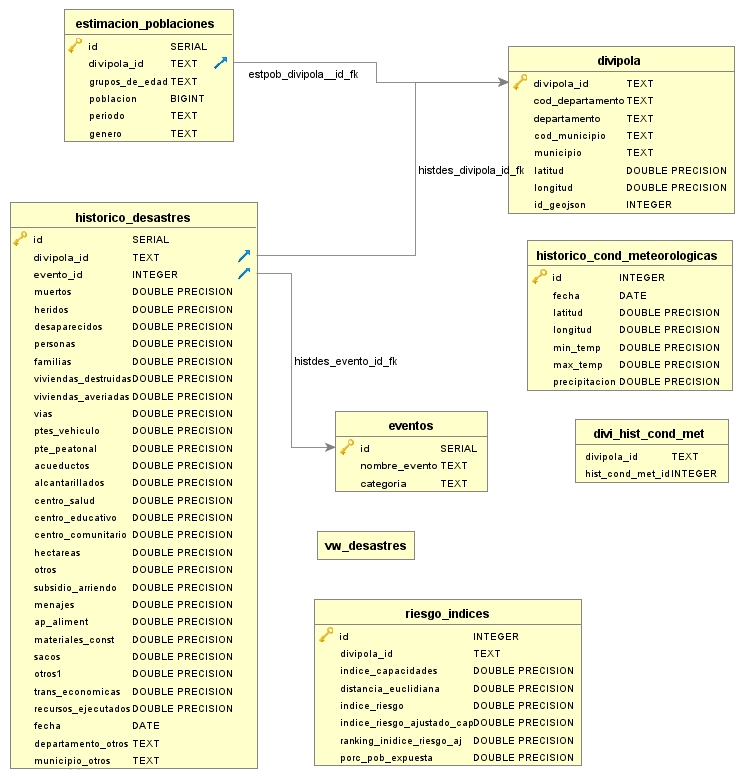
\includegraphics[width=0.95\textwidth]
{Project_Group03_ERModel}}
\caption{Entity relationship model.}
\label{fig:er_model}
\end{figure}

Figure \ref{fig:awsConnection} shows the database uploaded to AWS, and Figure \ref{fig:databaseLoaded} shows the database loaded to the AWS hosted database. The link between the front-end and the AWS-hosted databased was also stablished (see Figure \ref{fig:linkDASH_AWS}). 


\begin{figure}[!htb]
\center{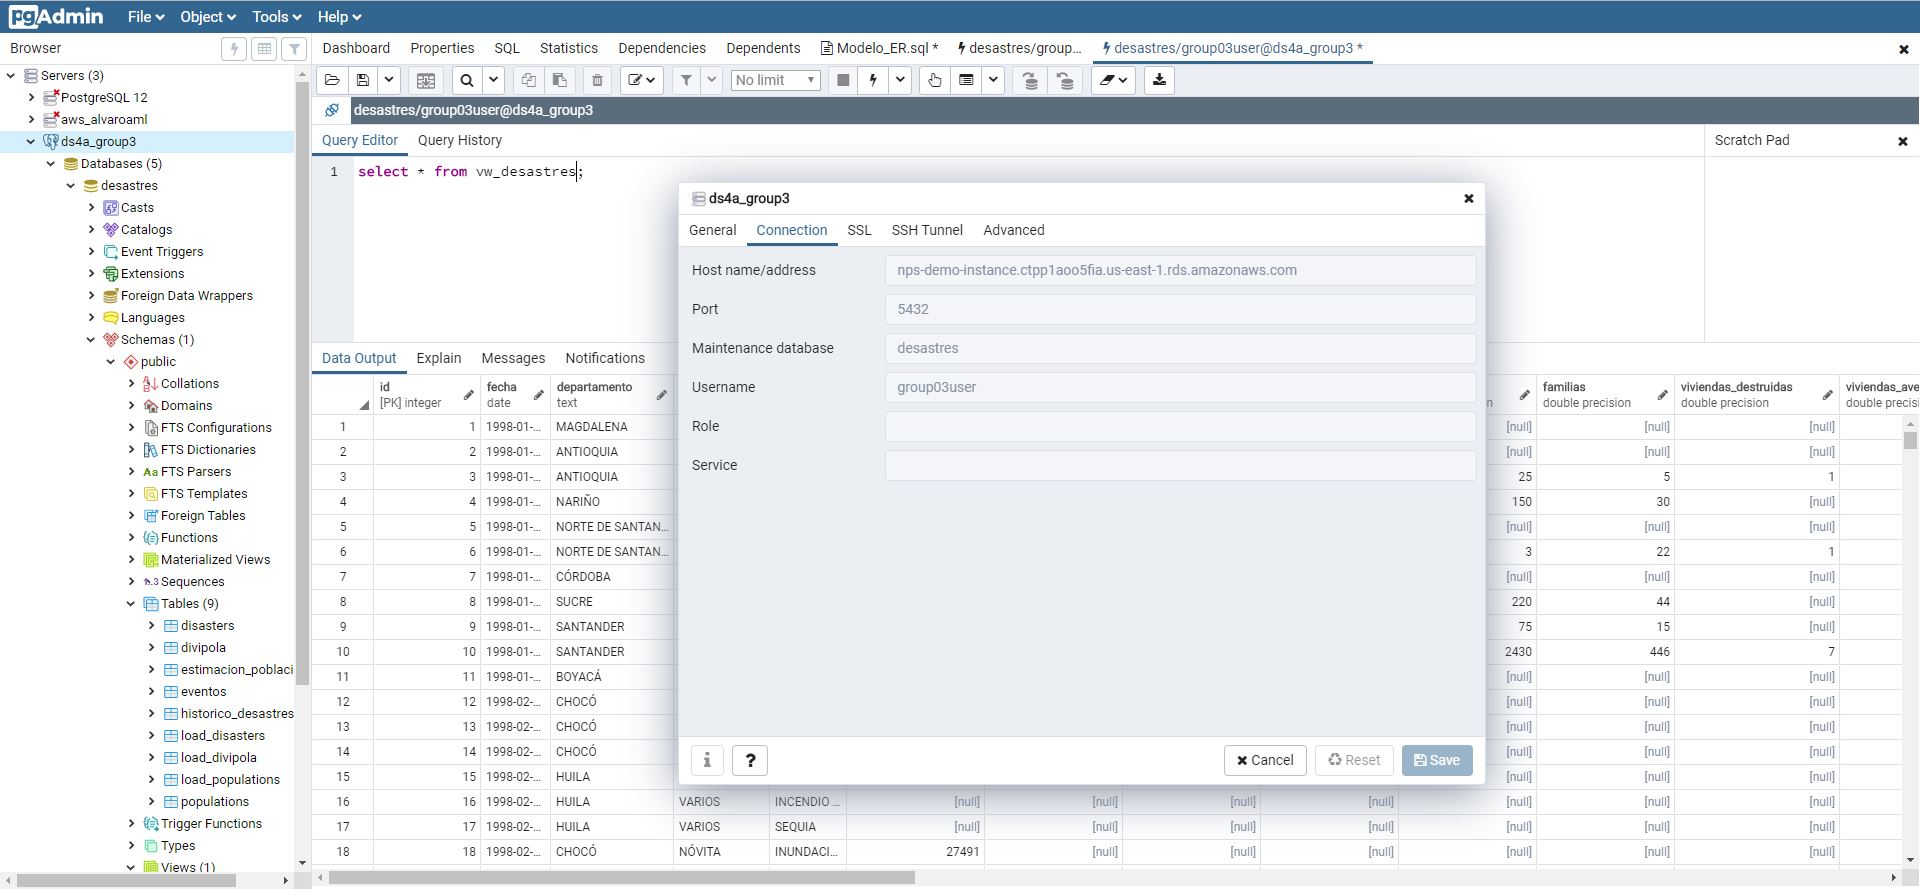
\includegraphics[width=0.95\textwidth]
{Desastres_AWS_Connection}}
\caption{AWS connection.}
\label{fig:awsConnection}
\end{figure}




\begin{figure}[!htb]
\center{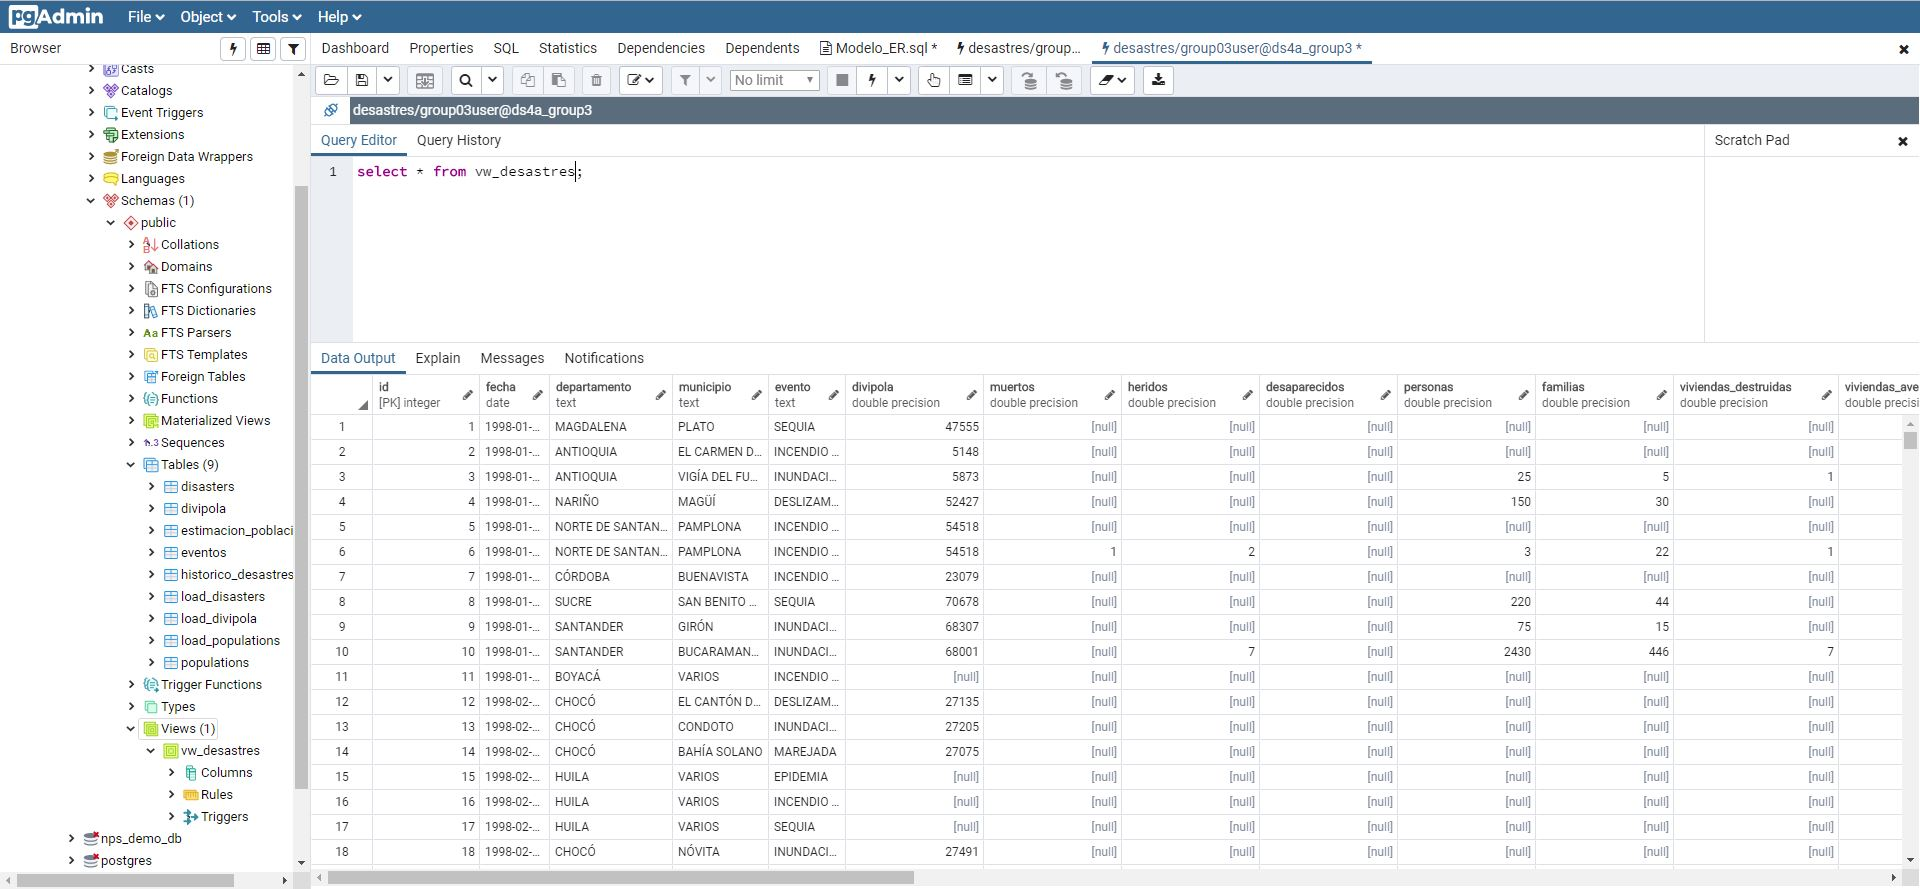
\includegraphics[width=0.95\textwidth]
{Desastres_data}}
\caption{Database loaded to AWS.}
\label{fig:databaseLoaded}
\end{figure}



\begin{figure}[!htb]
\center{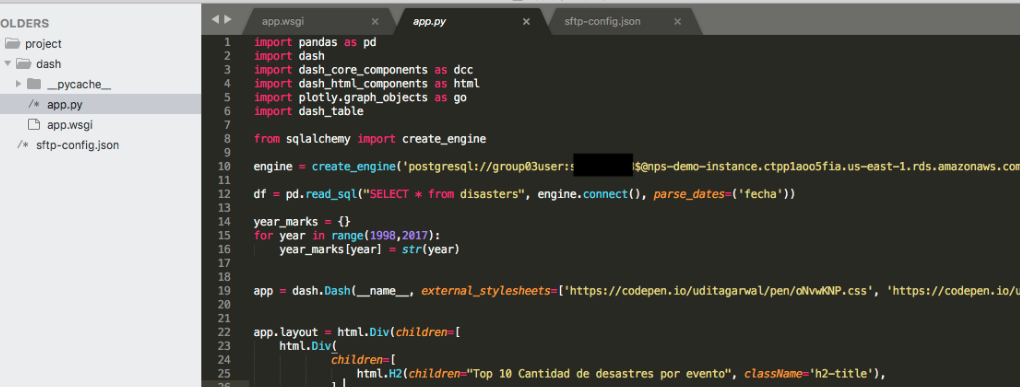
\includegraphics[width=0.95\textwidth]
{link_dash_aws}}
\caption{Link between DASH and AWS stablished}
\label{fig:linkDASH_AWS}
\end{figure}




\subsection{Interaction with the Dashboard}

Figure \ref{fig:page} shows what it looks like when you go to the website and click explore. Figure \ref{fig:MP} corresponds to the main view. On the left-hand side is dominated by a map where you see the municipalities with their Adjusted Risk Index, reflecting each city's built-up capabilities to cope with risk. That's by default but you can pick different variables for the heatmap.

In the upper right, the main view shows the possibility to drill down into impact variables: Affected people and families, affected and destroyed homes, and off course the deceased. Which accounts for the current vulnerability of the region of interest at any point in the last 30 years (which can be modified with the slider below the map).

Once a person has clicked on the region of interest, the Map changes and shows the selected division and the different subdivisions, as shown in Figure \ref{fig:MP_2}. The figure shows El Tarra Norte de Santander, a municipality with a population of around 11K located at Colombia's north east. Heavily impacted by and - ill prepared to deal with- hydro-meteorological events, which you can see from their vulnerability index and the trend in affected people and homes. 

If you check the evolution of average max temperatures you can see the size of the problem: Between 1990 and 2000 this indicator reached 29 degrees only once, in 1995. Then in 2001 it reached 29.17 and then again it stayed below 29 until 2010. Roughly a 10 year's cycle. However, it reached 29 again only 3 years later and hit a historical maximum at 29.23 in 2014. Stayed there for the next two years until 2016. You can also see how the minimum value for the last 10 years cycle is considerably higher than in the past.

Tipping points are crucial in environmental data. If earth's temperature is to rise 1.5 degrees, global population will be highly expose to severe heat waves, to Water Scarcity, and to flooding from sea level rise.



\begin{figure}%
\centering
\subfigure[Main page]{%
\label{fig:MP}%
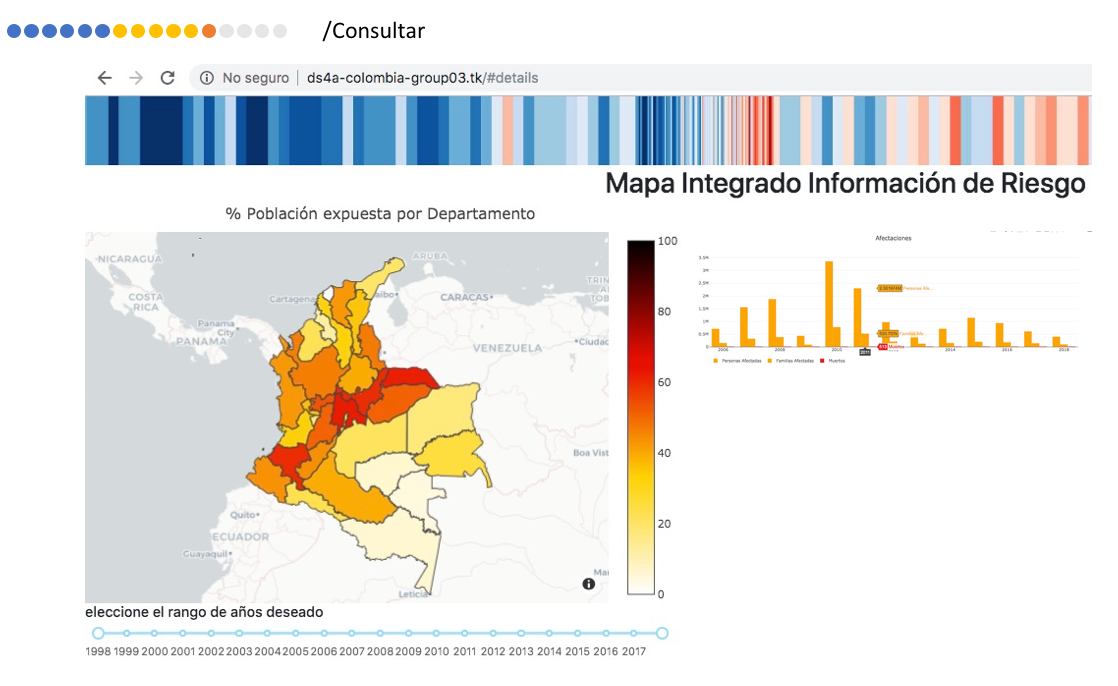
\includegraphics[height=3.5in, width=6in]{02_Home_mapa.png}}%
\qquad
\subfigure[Information of political division and subdivision]{%
\label{fig:MP_2}%
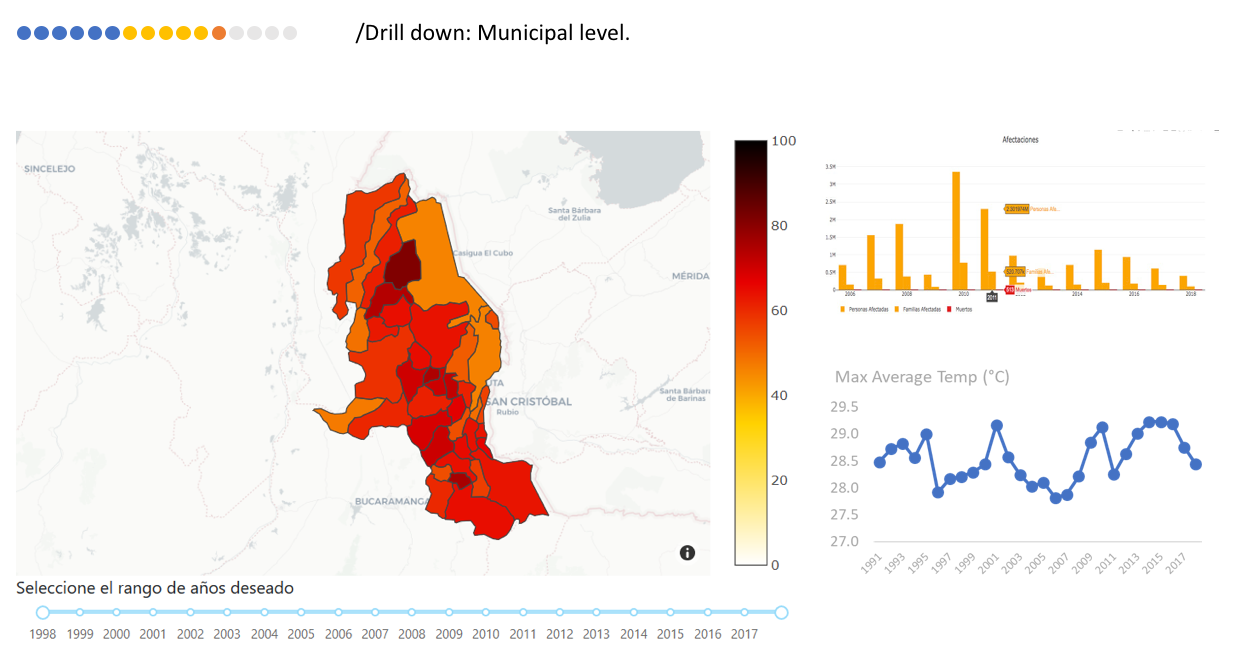
\includegraphics[height=3.5in, width=6in]{elTarra1.png}}%
%\subfigure[]{%
%\label{fig:second}%
%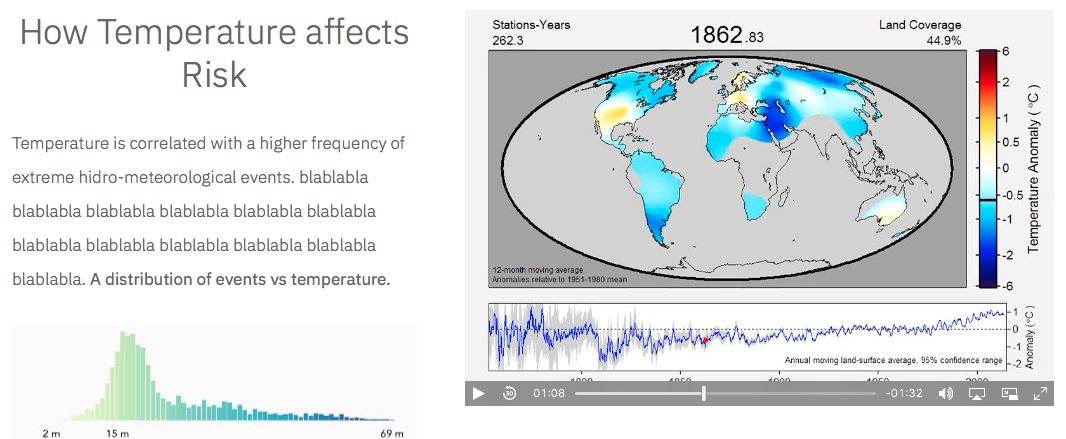
\includegraphics[height=2in, width=3in]{riesgo6}}%
\caption{Interacting with the Integrated Map of Risk Information in Colombia. Figure \ref{fig:MP} shows the main page with the  map of Colombia with the Risk Index. It provides interactive options to get detail information of selected Municipalities, risk index and a projected temperature indicator. Figure \ref{fig:MP_2} shows the municipality of El Tarra Norte de Santander, heavily impacted by hydrometeorological events with a hight vulnerability index and high number of people and home affected by those events.} 

\label{fig:page}%
\end{figure}


